\documentclass[12pt,a4paper,oneside]{report}

\usepackage[fontsize=13pt]{fontsize}

\usepackage{fontspec}
\usepackage{polyglossia}
\setdefaultlanguage{vietnamese}
\setmainfont{Times New Roman}
\DeclareMathSizes{13}{12}{9}{6}

\usepackage[
  a4paper,
  top=2.0cm,
  bottom=2.0cm,
  left=3.0cm,
  right=2.0cm,
  headheight=16pt
]{geometry}
\usepackage{setspace}
\setstretch{1.30}
\setlength{\parskip}{6pt}
\setlength{\emergencystretch}{2em}

\usepackage{graphicx}
\graphicspath{{img/}}
\usepackage{booktabs}
\usepackage{tabularx}
\usepackage{array}
\usepackage{enumitem}
\usepackage{caption}
\usepackage{float}
\usepackage{xcolor}
\usepackage{tikz}
\usetikzlibrary{arrows.meta,positioning,calc}
\usepackage{titlesec}
\usepackage{indentfirst}
\setlength{\parindent}{1cm}
\usepackage{fancyhdr}
\usepackage{hyperref}
\usepackage{xurl}
\urlstyle{same}

\hypersetup{
  hidelinks,
  pdftitle={Báo cáo Thực tập Kỹ thuật - Mai Duy Hiếu},
  pdfauthor={Mai Duy Hiếu}
}

\captionsetup{font=small,labelfont=bf,labelsep=colon}
\renewcommand{\figurename}{Hình}
\renewcommand{\tablename}{Bảng}
\renewcommand{\contentsname}{MỤC LỤC}
\renewcommand{\bibname}{TÀI LIỆU THAM KHẢO}
\gappto\captionsvietnamese{%
  \renewcommand{\listfigurename}{DANH MỤC HÌNH VẼ}%
  \renewcommand{\listtablename}{DANH MỤC BẢNG}%
}
\setcounter{tocdepth}{1}
\makeatletter
\renewcommand*\l@table{\@dottedtocline{1}{1.5em}{3em}}
\makeatother

\titleformat{\chapter}[display]
  {\normalfont\bfseries\centering\fontsize{16}{20}\selectfont}
  {CHƯƠNG \thechapter}{0.4em}{\MakeUppercase}
\titlespacing{\chapter}{0pt}{-18pt}{18pt}
\titleformat{\section}
  {\normalfont\bfseries\fontsize{14}{18}\selectfont}
  {\thesection}{0.6em}{}
\titlespacing{\section}{0pt}{18pt}{12pt}
\titleformat{\subsection}
  {\normalfont\itshape\fontsize{13}{17}\selectfont}
  {\thesubsection}{0.6em}{}
\titlespacing{\subsection}{0pt}{12pt}{12pt}

\pagestyle{fancy}
\fancyhf{}
\fancyfoot[C]{\thepage}
\renewcommand{\headrulewidth}{0pt}
\renewcommand{\footrulewidth}{0pt}
\fancypagestyle{plain}{
  \fancyhf{}
  \fancyfoot[C]{\thepage}
  \renewcommand{\headrulewidth}{0pt}
}



\newcommand{\StudentName}{Mai Duy Hiếu}
\newcommand{\StudentId}{20223967}
\newcommand{\StudentClass}{767288}
\newcommand{\StudentDob}{12/09/2004}
\newcommand{\StudentMajor}{Kỹ thuật Điện tử Viễn thông}
\newcommand{\UniversitySupervisor}{TS. Nguyễn Tiến Đạt}
\newcommand{\CompanySupervisor}{Nguyễn Hồng Sơn}
\newcommand{\CompanyRepresentative}{Nguyễn Thế Tài}
\newcommand{\CompanyName}{Công ty Cổ phần TECHPAL}
\newcommand{\CompanyAddress}{D48-13 Khu đô thị Geleximco, đường Lê Trọng Tấn, phường Dương Nội, Hà Nội}
\newcommand{\InternshipPeriod}{20/07/2026 -- 28/08/2026}
\newcommand{\Semester}{2025.3 -- năm học 2025--2026}
\newcommand{\ReportTopic}{Tìm hiểu quy trình lựa chọn linh kiện điện tử và thiết bị tự động hóa tại Công ty Cổ phần TECHPAL}

\begin{document}

\hypersetup{pageanchor=false}
% Trang bìa căn theo tâm vật lý của giấy A4; phần ruột dùng hai lề bên bằng nhau.
\newgeometry{top=2cm,bottom=2cm,left=2cm,right=2cm}
\begin{titlepage}
\thispagestyle{empty}
\begin{tikzpicture}[remember picture,overlay]
  \draw[line width=1.0pt]
    ($(current page.north west)+(1.55cm,-1.35cm)$)
    rectangle
    ($(current page.south east)+(-1.55cm,1.35cm)$);
  \draw[line width=0.4pt]
    ($(current page.north west)+(1.63cm,-1.43cm)$)
    rectangle
    ($(current page.south east)+(-1.63cm,1.43cm)$);
\end{tikzpicture}
\begin{center}
  {\bfseries\fontsize{21}{26}\selectfont
  ĐẠI HỌC BÁCH KHOA HÀ NỘI\\
  TRƯỜNG ĐIỆN -- ĐIỆN TỬ\par}

  \vspace{0.15cm}
  \rule{6cm}{0.4pt}

  \vspace{0.8cm}
  
\includegraphics[height=4.8cm]{logo.png}

  \vspace{0.7cm}
  {\bfseries\fontsize{21}{26}\selectfont BÁO CÁO\\[0.25cm]
  THỰC TẬP KỸ THUẬT\par}

  \vspace{1.0cm}
  {\bfseries\fontsize{21}{26}\selectfont\MakeUppercase{\CompanyName}\par}

  \vfill

  \begin{tabular}{@{}>{\bfseries}l@{\hspace{1.2em}}l@{}}
    Giảng viên hướng dẫn: & \UniversitySupervisor \\
    Sinh viên thực hiện: & \StudentName \\
    MSSV: & \StudentId \\
    Mã lớp học: & \StudentClass \\
  \end{tabular}

  \vfill
  {\bfseries Hà Nội, 8/2026}
\end{center}
\end{titlepage}
\restoregeometry

\hypersetup{pageanchor=true}

\pagenumbering{roman}
\setcounter{page}{1}
\chapter*{LỜI NÓI ĐẦU}
\addcontentsline{toc}{chapter}{LỜI NÓI ĐẦU}

Thực tập kỹ thuật là học phần giúp sinh viên kết nối kiến thức cơ sở ngành với
môi trường làm việc thực tế. Đối với ngành Kỹ thuật Điện tử Viễn thông, việc
tiếp cận linh kiện điện tử, thiết bị tự động hóa, tài liệu kỹ thuật và quy trình
lựa chọn giải pháp có ý nghĩa quan trọng trong quá trình hình thành tư duy kỹ
sư. Đây cũng là cơ hội để sinh viên rèn luyện tác phong làm việc, kỹ năng tìm
kiếm thông tin, đọc tài liệu chuyên ngành và trình bày kết quả kỹ thuật.

Trong học kỳ \Semester, em thực hiện học phần Thực tập Kỹ thuật tại
\CompanyName, dưới sự hướng dẫn tại đơn vị của anh \CompanySupervisor\ và sự
hướng dẫn của giảng viên \UniversitySupervisor. Báo cáo tập trung giới thiệu
khái quát doanh nghiệp, các lĩnh vực hoạt động có liên quan đến chuyên ngành,
đồng thời hệ thống hóa nội dung tìm hiểu về linh kiện điện tử và thiết bị tự
động hóa.

Thuận lợi lớn nhất là \CompanyName\ có danh mục linh kiện điện tử và thiết bị
tự động hóa khá đa dạng, kèm trang giới thiệu và trang bán hàng công khai. Nhờ
đó em có thể đối chiếu mô tả sản phẩm với datasheet của hãng, đồng thời được
anh \CompanySupervisor\ và giảng viên \UniversitySupervisor\ định hướng phạm vi
tìm hiểu cho sát chuyên ngành. Khó khăn chủ yếu đến từ thời gian thực tập
ngắn, danh mục mã hàng lớn và cách đặt mã khác nhau giữa các hãng. Em cũng
không tiếp cận được quy trình nội bộ, dữ liệu kho hay phòng thí nghiệm để đo
kiểm, nên phần phân tích ứng dụng trong báo cáo mới dừng ở mức phương án trên
giấy. Việc đọc tài liệu tiếng Anh và không bỏ sót hậu tố, kiểu vỏ, dải nhiệt độ
hay trạng thái vòng đời cũng đòi hỏi em phải tra cứu nhiều lần mới quen.


Em xin chân thành cảm ơn Ban lãnh đạo \CompanyName, anh \CompanySupervisor,
giảng viên \UniversitySupervisor\ cùng các cá nhân đã hỗ trợ em trong quá trình
thực hiện học phần.

\clearpage
\tableofcontents
\clearpage
\phantomsection
\addcontentsline{toc}{chapter}{\listfigurename}
\listoffigures
\clearpage
\phantomsection
\addcontentsline{toc}{chapter}{\listtablename}
\listoftables
\clearpage

\pagenumbering{arabic}
\setcounter{page}{1}
\chapter{GIỚI THIỆU ĐƠN VỊ THỰC TẬP}

\section{Thông tin chung}

\CompanyName\ (tên quốc tế: \textit{TECHPAL Joint Stock Company}, viết tắt
TECHPAL., JSC) có mã số thuế 0104469357, thành lập từ ngày 08/02/2010
\cite{techpal-intro}. Địa chỉ
văn phòng giao dịch đặt tại \CompanyAddress. Số điện thoại liên hệ là 024 3793
8272, email \href{mailto:info@techpal.vn}{info@techpal.vn}, website
\url{https://techpal.vn}.

\begin{table}[H]
\centering
\caption{Thông tin khái quát về đơn vị thực tập}
\label{tab:company-info}
\begin{tabularx}{\textwidth}{>{\bfseries}p{4.3cm}X}
\toprule
Tên doanh nghiệp & Công ty Cổ phần TECHPAL \\
Tên quốc tế & TECHPAL Joint Stock Company \\
Tên viết tắt & TECHPAL., JSC \\
Mã số thuế & 0104469357 \\
Ngày thành lập & 08/02/2010 \\
Trụ sở chính & \CompanyAddress \\
Website & \url{https://techpal.vn} \\
Người hướng dẫn & \CompanySupervisor \\
Đại diện xác nhận & \CompanyRepresentative, Phó Tổng giám đốc \\
Thời gian thực tập & \InternshipPeriod \\
\bottomrule
\end{tabularx}
\end{table}

\section{Quá trình hình thành và định hướng phát triển}

Trên website chính thức, TECHPAL giới thiệu bốn mảng hoạt động chính gồm: kinh
doanh linh kiện điện tử và thiết bị tự động hóa; nghiên cứu, chuyển giao công
nghệ; năng lượng xanh (chủ yếu là điện mặt trời); và đầu tư nông nghiệp công
nghệ cao \cite{techpal-intro}. Nhìn chung, công ty xuất phát từ lĩnh vực điện --
điện tử rồi mở rộng thêm sang năng lượng và nông nghiệp.

Về định hướng, TECHPAL tập trung vào đổi mới công nghệ và phát triển bền vững.
Công ty đã triển khai một số dự án điện mặt trời áp mái, song song với hoạt động
cung ứng thiết bị tự động hóa và các dự án nông nghiệp ứng dụng công nghệ
\cite{techpal-intro}.

\section{Lĩnh vực hoạt động chuyên môn}

\subsection{Linh kiện điện tử và thiết bị tự động hóa}

Trên trang bán hàng của TECHPAL, sản phẩm được chia thành bốn nhóm: linh kiện
điện tử, thiết bị tự động hóa công nghiệp, vật tư phụ trợ và thiết bị phòng sạch.
Em thấy trên danh mục có khá nhiều mã linh kiện bán dẫn, đầu nối, rơ-le, nguồn
cấp, cảm biến, bộ điều khiển PLC, mô-đun vào/ra và bộ ghi dữ liệu
\cite{techpal-components}.

Việc cung ứng linh kiện kỹ thuật không đơn giản chỉ là bán hàng. Người làm kỹ
thuật phải đọc đúng mã linh kiện, so sánh thông số điện và cơ khí, kiểm tra xem
có thay thế được không, xem sản phẩm còn được sản xuất hay đã ngừng, rồi cả
điều kiện lưu kho, vận chuyển và chống tĩnh điện nữa. Bỏ sót bước nào cũng có
thể gây ra lỗi cho hệ thống về sau.

\subsection{Nghiên cứu và chuyển giao công nghệ}

Mảng R\&D của TECHPAL hoạt động như cầu nối giữa yêu cầu thực tế và giải pháp
kỹ thuật. Quy trình thường bắt đầu từ khảo sát nhu cầu, sau đó phân rã chức
năng, chọn phần cứng, thiết kế kết nối, thử nghiệm rồi bàn giao. Với sinh viên
ngành Điện tử Viễn thông, đây là nơi có thể áp dụng các kiến thức về mạch điện,
vi điều khiển, cảm biến hay truyền thông công nghiệp.

\subsection{Năng lượng xanh và điện mặt trời}

Một hệ thống điện mặt trời thông thường gồm tấm pin, thiết bị bảo vệ DC, bộ
biến đổi (inverter), hệ thống giám sát và phần kết nối lưới. Khi chọn thiết bị
cho hệ thống này cần xét đến công suất, dải điện áp, hiệu suất, điều kiện thời
tiết và yêu cầu an toàn. TECHPAL có tham gia lĩnh vực này thông qua các dự án
điện mặt trời áp mái.

\subsection{Nông nghiệp công nghệ cao}

Mảng nông nghiệp công nghệ cao tạo ra nhu cầu về cảm biến môi trường, bộ điều
khiển, thiết bị truyền thông và lưu trữ dữ liệu. Tuy mục tiêu cuối cùng là phục
vụ sản xuất nông nghiệp, nhưng nhiều thiết bị cốt lõi vẫn thuộc lĩnh vực điện
tử và tự động hóa -- ví dụ như đo nhiệt độ, độ ẩm, điều khiển quạt, bơm hay thu
thập dữ liệu từ xa.

\section{Cơ cấu tổ chức}

Theo thông tin trên website, TECHPAL có cơ cấu gồm Đại hội đồng cổ đông, Hội
đồng quản trị, Ban Kiểm soát, Ban Tổng giám đốc và các phòng chuyên môn
\cite{techpal-intro}. Cụ thể,
các phòng ban được liệt kê gồm: Kinh doanh linh kiện điện tử, Tài chính -- Kế
toán, Hành chính -- Tổng hợp, Phát triển và vận hành dự án, Pháp chế doanh
nghiệp. Ngoài ra còn có đơn vị thành viên, văn phòng đại diện và các ban quản lý
dự án. Bài đăng về Đại hội đồng cổ đông thường niên năm
2026 cũng xác nhận ông \CompanyRepresentative\ giữ chức Thành viên Hội đồng quản
trị kiêm Phó Tổng giám đốc \cite{techpal-agm2026}.

\section{Các vị trí công việc và yêu cầu năng lực}

Từ các lĩnh vực hoạt động nêu trên, em tạm chia ra một số nhóm vị trí liên quan
đến chuyên ngành Điện tử Viễn thông như trong Bảng~\ref{tab:positions}. Cần lưu ý
đây là cách em tự phân nhóm dựa trên tính chất công việc, không phải danh sách
tuyển dụng chính thức của công ty.

\begin{table}[htbp]
\centering
\caption{Một số nhóm vị trí và năng lực cần thiết}
\label{tab:positions}
\small
\renewcommand{\arraystretch}{1.08}
\begin{tabularx}{\textwidth}{>{\raggedright\arraybackslash}p{3.1cm}
                  >{\raggedright\arraybackslash}X
                  >{\raggedright\arraybackslash}X}
\toprule
\textbf{Nhóm vị trí} & \textbf{Nhiệm vụ điển hình} & \textbf{Kiến thức, kỹ năng cần có} \\
\midrule
Kỹ sư ứng dụng linh kiện & Đọc yêu cầu, chọn linh kiện, kiểm tra khả năng thay thế và hỗ trợ kỹ thuật & Mạch điện tử, đọc datasheet, tra cứu mã hàng, giao tiếp kỹ thuật \\
\addlinespace
Kỹ sư tự động hóa & Lựa chọn PLC, cảm biến, cơ cấu chấp hành; cấu hình và kiểm thử hệ thống & Điều khiển, điện công nghiệp, PLC/HMI, truyền thông công nghiệp \\
\addlinespace
Kỹ sư dự án & Khảo sát, lập phương án, bóc tách thiết bị, theo dõi triển khai & Tư duy hệ thống, đọc bản vẽ, lập kế hoạch, quản lý rủi ro \\
\addlinespace
Kỹ sư R\&D & Phân tích yêu cầu, thiết kế nguyên mẫu, đo kiểm và lập tài liệu & Điện tử tương tự -- số, vi điều khiển, đo lường, thiết kế và kiểm thử \\
\addlinespace
Kiểm tra kỹ thuật & Kiểm tra mã hàng, ngoại quan, thông số và hồ sơ chất lượng & Dụng cụ đo, tiêu chuẩn chất lượng, ESD, kỹ năng ghi nhận dữ liệu \\
\bottomrule
\end{tabularx}
\end{table}

\chapter{NỘI DUNG THỰC TẬP}

\section{Phạm vi và phương pháp tìm hiểu}

Trong thời gian thực tập, dưới sự hướng dẫn của anh \CompanySupervisor{}, em tập
trung tìm hiểu hoạt động cung ứng linh kiện điện tử và thiết bị tự động hóa tại
\CompanyName{}. Em chọn đi vào ba vấn đề chính: thứ nhất là mối liên hệ giữa các
bộ phận tham gia chuỗi cung ứng; thứ hai là cách chuyển yêu cầu của khách hàng
thành tiêu chí chọn thiết bị; và thứ ba là cách kiểm tra một mã hàng cụ thể bằng
tài liệu của nhà sản xuất.

Nguồn thông tin chủ yếu là website giới thiệu, trang bán hàng công khai của
TECHPAL và tài liệu kỹ thuật (datasheet) từ các hãng sản xuất. Em chỉ sử dụng
những gì có thể tra cứu và kiểm chứng được, còn quy trình nội bộ, dữ liệu kho
hay kết quả đo kiểm thì em không có quyền truy cập. Các phân tích ứng dụng trong
chương này mới ở mức phương án trên giấy, chưa phải sản phẩm đã làm ra.

Em thực hiện theo bốn bước:

\begin{enumerate}[label=\arabic*)]
  \item Tìm các nhóm sản phẩm và bộ phận liên quan từ nguồn công khai;
  \item Chọn vài mã đại diện có trong danh mục của TECHPAL;
  \item Đối chiếu mô tả trên trang bán hàng với tài liệu chính thức của hãng;
  \item Tổng hợp lại thành quy trình lựa chọn, kèm một bài toán minh họa.
\end{enumerate}

\section{Các vị trí liên quan trong chuỗi cung ứng}

Trên trang giới thiệu của TECHPAL có đề cập đến ba bộ phận trực tiếp tham gia
cung ứng: Sale, Mua hàng Quốc tế và Logistics. Ba bộ phận
này phụ trách các giai đoạn khác nhau nhưng đều làm việc trên cùng một đơn hàng,
cùng mã linh kiện, số lượng, yêu cầu chất lượng và deadline giao hàng
\cite{techpal-about}.

\begin{table}[H]
\centering
\caption{Vai trò của các bộ phận trong chuỗi cung ứng linh kiện}
\label{tab:chapter2-roles}
\small
\renewcommand{\arraystretch}{1.1}
\begin{tabularx}{\textwidth}{>{\bfseries\raggedright\arraybackslash}p{3.1cm} >{\raggedright\arraybackslash}X >{\raggedright\arraybackslash}X}
\toprule
Bộ phận & Nội dung công việc liên quan & Kiến thức, kỹ năng cần thiết \\
\midrule
Sale & Tiếp nhận nhu cầu, làm rõ mã hàng, số lượng, ứng dụng và thời hạn; trao đổi phương án với khách hàng & Giao tiếp kỹ thuật, đọc mã linh kiện, hiểu thông số cơ bản và lập báo giá \\
Mua hàng Quốc tế & Tìm nguồn, kiểm tra khả năng cung ứng, quy cách đóng gói và chứng từ; làm việc với nhà cung cấp & Tiếng Anh chuyên ngành, tra cứu chéo, đánh giá nguồn và quản lý thay đổi sản phẩm \\
Logistics & Theo dõi vận chuyển, tiếp nhận, bảo quản và bàn giao; kiểm tra sự phù hợp giữa hàng hóa với chứng từ & Quản lý mã hàng, đóng gói, điều kiện lưu kho, ESD và truy xuất lô hàng \\
\bottomrule
\end{tabularx}
\end{table}

Bảng~\ref{tab:chapter2-roles} là do em tự tổng hợp theo tính chất công việc, không
phải bản mô tả nhân sự chính thức của công ty. Tuy nhiên, một điểm em thấy rõ là
với linh kiện điện tử, chỉ cần sai một hậu tố trong mã đặt hàng là có thể nhận
nhầm kiểu vỏ, dải nhiệt độ hay quy cách đóng gói. Cho nên thông tin kỹ thuật
cần phải được giữ nhất quán khi chuyển từ bộ phận này sang bộ phận khác.

Từ thông tin về dịch vụ đặt hàng qua châu Âu -- Mỹ, DigiKey, Mouser và Trung
Quốc trên trang TECHPAL \cite{techpal-about}, em vẽ lại luồng xử lý một
yêu cầu cung ứng như Hình~\ref{fig:supply-flow}. Sơ đồ này chỉ mang tính khái
quát để phục vụ học tập, không phải quy trình nội bộ mà công ty đang áp dụng.

\begin{figure}[H]
\centering
\begin{tikzpicture}[
  block/.style={draw, rounded corners=2pt, align=center, minimum height=1.25cm,
                text width=2.35cm, font=\small},
  line/.style={-{Latex[length=2.3mm]}, thick},
  node distance=0.45cm
]
  \node[block] (need) {Tiếp nhận\\yêu cầu};
  \node[block, right=of need] (normalize) {Chuẩn hóa\\mã và thông số};
  \node[block, right=of normalize] (source) {Tìm nguồn và\\đối chiếu};
  \node[block, right=of source] (order) {Đặt hàng,\\vận chuyển};
  \node[block, right=of order] (deliver) {Tiếp nhận và\\bàn giao};
  \draw[line] (need) -- (normalize);
  \draw[line] (normalize) -- (source);
  \draw[line] (source) -- (order);
  \draw[line] (order) -- (deliver);
\end{tikzpicture}
\caption{Luồng xử lý yêu cầu cung ứng (mô hình hóa từ thông tin công khai)}
\label{fig:supply-flow}
\end{figure}

\section{Khảo sát danh mục sản phẩm của TECHPAL}

Danh mục trực tuyến của TECHPAL chia sản phẩm thành bốn nhóm lớn: linh kiện điện
tử; thiết bị tự động hóa công nghiệp; vật tư phụ trợ công nghiệp; và thiết bị,
vật tư phòng sạch. Cách phân nhóm này
giúp thu hẹp phạm vi tìm kiếm, nhưng chỉ nhìn vào tên nhóm thì chưa biết được
sản phẩm có hợp với ứng dụng cụ thể hay không \cite{techpal-components}.

\begin{table}[H]
\centering
\caption{Các nhóm cung ứng chính trên danh mục TECHPAL}
\label{tab:techpal-categories}
\small
\renewcommand{\arraystretch}{1.1}
\begin{tabularx}{\textwidth}{>{\bfseries\raggedright\arraybackslash}p{4.1cm} >{\raggedright\arraybackslash}X >{\raggedright\arraybackslash}X}
\toprule
Nhóm cung ứng & Thành phần tiêu biểu quan sát được & Thông tin cần kiểm tra \\
\midrule
Linh kiện điện tử & IC, vi điều khiển, linh kiện công suất, đầu nối, rơ-le, màn hình & Mã đầy đủ, kiểu vỏ, điện áp, dòng, nhiệt độ và trạng thái vòng đời \\
Thiết bị tự động hóa & Mô-đun PLC/I/O, cảm biến, encoder, bộ nguồn, thiết bị ghi dữ liệu & Kiến trúc hệ thống, số kênh, loại tín hiệu, giao thức và khả năng mở rộng \\
Vật tư phụ trợ công nghiệp & Đầu nối, dây dẫn, phụ kiện lắp đặt và vật tư bảo trì & Kích thước, vật liệu, điều kiện môi trường và tương thích cơ khí \\
Thiết bị, vật tư phòng sạch & Dụng cụ và vật tư phục vụ môi trường kiểm soát bụi bẩn & Cấp sạch, vật liệu, quy cách đóng gói và yêu cầu sử dụng \\
\bottomrule
\end{tabularx}
\end{table}

Để không dừng lại ở mô tả chung chung, em chọn bốn mã hàng có thật trong danh
mục TECHPAL \cite{techpal-components} để tra cứu kỹ hơn. Bốn mã này đại diện cho bốn loại thiết bị khác
nhau: IC truyền thông, mô-đun I/O công nghiệp, thiết bị kết nối I/O phân tán và
bộ ghi dữ liệu.

\begin{table}[H]
\centering
\caption{Một số mã hàng đại diện trong danh mục TECHPAL}
\label{tab:representative-products}
\small
\renewcommand{\arraystretch}{1.1}
\begin{tabularx}{\textwidth}{>{\ttfamily\raggedright\arraybackslash}p{4.1cm} >{\raggedright\arraybackslash}p{2.8cm} >{\raggedright\arraybackslash}X}
\toprule
\normalfont\textbf{Mã sản phẩm} & \textbf{Nhóm chức năng} & \textbf{Mô tả dùng cho bước tra cứu} \\
\midrule
MAX487CSA+T & IC truyền thông & Bộ thu phát RS-485/RS-422 công suất thấp, vỏ SOIC 8 chân \\
BMXAMI0410 & Mô-đun vào tương tự & Mô-đun Modicon X80 có bốn ngõ vào tương tự tốc độ cao \\
6ES7153-1AA03-0XB0 & Giao tiếp I/O phân tán & Mô-đun kết nối SIMATIC DP IM 153-1 cho ET 200M \\
CR1000X & Đo lường và lưu trữ & Bộ ghi dữ liệu có khả năng đo, xử lý, lưu trữ và truyền thông \\
\bottomrule
\end{tabularx}
\end{table}

\section{Quy trình đọc và lựa chọn thiết bị}

\subsection{Chuẩn hóa yêu cầu đầu vào}

Nếu khách hàng chỉ nói ``cần IC RS-485'' hay ``cần mô-đun analog'' thì chưa đủ
thông tin để đặt hàng. Yêu cầu như vậy cần được cụ thể hóa thành: chức năng gì,
điện áp bao nhiêu, mấy kênh, loại tín hiệu, tốc độ, giao thức, nhiệt độ làm
việc, kiểu lắp, số lượng và khi nào cần. Nếu đây là mã thay thế cho linh kiện
cũ thì phải có thêm mã gốc và thông tin về bo mạch đang sử dụng.

\subsection{Kiểm tra mã và tài liệu kỹ thuật}

Mã hàng cần đọc đầy đủ kể cả hậu tố -- điểm này ban đầu em cũng hay bỏ qua.
Để xác nhận thông số, nguồn đáng tin nhất là trang sản phẩm và datasheet của nhà
sản xuất. Mô tả trên website nhà cung ứng giúp định vị nhanh sản phẩm, nhưng
không nên dựa vào đó để kết luận tương thích hay không. Các bước kiểm tra em đề
xuất gồm:

\begin{enumerate}[label=\arabic*)]
  \item Xác nhận nhà sản xuất và mã đặt hàng đầy đủ;
  \item Đối chiếu chức năng, sơ đồ chân hoặc kiến trúc mô-đun;
  \item Kiểm tra giới hạn điện, nhiệt và điều kiện làm việc khuyến nghị;
  \item Xem kiểu vỏ, kích thước, đầu nối và cách lắp đặt;
  \item Xác định trạng thái vòng đời: còn sản xuất hay chỉ còn dạng phụ tùng;
  \item Lưu lại link tài liệu, ngày tra cứu và kết luận.
\end{enumerate}

Kết quả tra cứu nên ghi lại dưới dạng bảng kiểm để sau này người khác có thể
xem lại được nguồn dữ liệu và lý do chọn. Bảng~\ref{tab:technical-checklist}
liệt kê những câu hỏi tối thiểu cần trả lời trước khi đề xuất mua một mã hàng.

\begin{table}[H]
\centering
\caption{Bảng kiểm kỹ thuật trước khi lựa chọn mã hàng}
\label{tab:technical-checklist}
\footnotesize
\renewcommand{\arraystretch}{1.0}
\begin{tabularx}{\textwidth}{>{\bfseries\raggedright\arraybackslash}p{3.4cm} >{\raggedright\arraybackslash}X >{\raggedright\arraybackslash}X}
\toprule
Nội dung kiểm tra & Câu hỏi cần trả lời & Rủi ro nếu bỏ sót \\
\midrule
Định danh & Mã, hậu tố và hãng đã chính xác chưa? & Nhận sai biến thể hoặc sai quy cách đóng gói \\
Thông số điện & Điện áp, dòng, mức logic và công suất có phù hợp? & Hỏng linh kiện hoặc hệ thống hoạt động không ổn định \\
Giao tiếp & Chuẩn vật lý, giao thức và tốc độ có tương thích? & Không trao đổi được dữ liệu \\
Cơ khí & Vỏ, chân, đầu nối và kích thước lắp có khớp? & Không lắp được hoặc phải sửa thiết kế \\
Môi trường & Nhiệt độ, độ ẩm, rung và cấp bảo vệ có đáp ứng? & Suy giảm độ tin cậy khi vận hành \\
Vòng đời & Sản phẩm còn sản xuất hay chỉ còn dạng phụ tùng? & Khó mua bổ sung và tăng chi phí bảo trì \\
Chứng từ & Datasheet, nguồn gốc, lô hàng và chứng nhận có đủ? & Khó truy xuất và nghiệm thu \\
\bottomrule
\end{tabularx}
\end{table}

\subsection{Đánh giá khả năng thay thế}

Hai sản phẩm có cùng tên chức năng chưa chắc đã thay thế được cho nhau. Với IC
thì phải so chân, mức điện, tốc độ, tải bus, vỏ và dải nhiệt độ. Với mô-đun
công nghiệp thì còn phải xem rack, bộ điều khiển đi kèm, phiên bản firmware, cấu
hình I/O và chứng nhận. Đặc biệt khi sản phẩm đã ngừng sản xuất (chỉ còn dạng
phụ tùng), chi phí thay thế phải tính cả việc chuyển đổi hệ thống chứ không chỉ
nhìn giá mô-đun.

\section{Phân tích một số mã sản phẩm đại diện}

\subsection{Bộ thu phát MAX487CSA+T}

Trên trang TECHPAL, MAX487CSA+T được liệt kê trong nhóm linh kiện điện tử, mô
tả là bộ thu phát bán song công, vỏ SOIC 8 chân \cite{techpal-max487}. Em tra
trên trang Analog Devices thì thấy MAX487 là IC thu phát RS-485/RS-422 nguồn đơn
5~V, phiên bản giới hạn tốc độ sườn, hỗ trợ tới 250~kbps. Đầu vào thu có tải
$1/4$ đơn vị nên về lý thuyết có thể nối tối đa 128 nút trên một bus
\cite{adi-max487}.

Nếu dùng MAX487CSA+T cho giao tiếp nối tiếp trong thiết kế nhúng thì cần kiểm
tra thêm mấy thứ: điện áp logic phía vi điều khiển có tương thích 5~V không,
đường truyền có cần điện trở kết thúc không, bus cần phân cực ra sao, có cần bảo
vệ ESD không, và nếu hai đầu chênh lệch điện thế đất thì có cần cách ly không.
Ngoài ra, hậu tố ``T'' liên quan tới quy cách đóng gói (tape and reel) nên khi
đặt mua không được bỏ.

\subsection{Mô-đun vào tương tự BMXAMI0410}

Mã BMXAMI0410 trên TECHPAL thuộc nhóm thiết bị tự động hóa. Theo Schneider
Electric, đây là mô-đun Modicon X80 với bốn ngõ vào analog tốc độ cao
\cite{schneider-bmxami0410}. Khác với một IC rời, mô-đun này không thể dùng
đơn lẻ mà phụ thuộc vào cả hệ thống: rack nào tương thích, CPU PLC nào, cảm
biến ra kiểu tín hiệu gì, đấu dây thế nào, phần mềm cấu hình ra sao.

Điều em rút ra ở đây là trong cung ứng tự động hóa, số kênh hay loại tín hiệu
mới chỉ là điều kiện cần. Muốn chốt mã thì phải xem thêm tài liệu tương thích
hệ thống và phụ kiện đầu nối. Giả sử khách hàng chỉ nói ``cho mô-đun analog bốn
kênh'', bên kỹ thuật hoặc Sale cần hỏi thêm đang dùng PLC/rack gì và đo tín
hiệu dải nào.

\subsection{Mô-đun Siemens 6ES7153-1AA03-0XB0}

TECHPAL có bán mã 6ES7153-1AA03-0XB0. Tra trên trang Siemens, em thấy đây là
mô-đun kết nối SIMATIC DP IM~153-1 dùng cho trạm ET~200M, hỗ trợ tối đa tám
mô-đun S7-300. Điểm đáng chú ý là mã này hiện tại Siemens phân loại là
\textit{phụ tùng} (spare part only) \cite{siemens-im153}.

Trạng thái phụ tùng ảnh hưởng rất lớn đến quyết định mua. Nếu nhà máy đang chạy
hệ thống cũ và cần thay thế để giảm thời gian dừng máy thì vẫn phải mua mã này.
Nhưng nếu làm dự án mới thì nên cân nhắc nền tảng khác có vòng đời dài hơn. Em
nghĩ đây là ví dụ rõ nhất cho thấy kiểm tra vòng đời quan trọng không kém kiểm
tra thông số kỹ thuật.

\subsection{Bộ ghi dữ liệu CR1000X}

TECHPAL liệt kê CR1000X của Campbell Scientific trong nhóm thiết bị tự động hóa,
mô tả là bộ lưu trữ xử lý dữ liệu. Tài liệu hãng cho
biết CR1000X có 16 đầu vào analog đơn (hoặc 8 vi sai), ADC 24 bit, và tích hợp
sẵn khả năng đo cảm biến, xử lý, lưu trữ lẫn truyền dữ liệu
\cite{techpal-cr1000x,campbell-cr1000x}.

CR1000X khá phù hợp cho các bài toán thu thập dữ liệu môi trường hay trạm đo
từ xa. Tuy vậy, không phải cứ thấy 16 kênh là đủ. Người chọn thiết bị phải xem
kỹ: loại cảm biến, dải đo, độ chính xác cần thiết, chu kỳ lấy mẫu, bộ nhớ, cổng
giao tiếp, nguồn cấp và điều kiện ngoài trời hay trong nhà. Hãng cũng khuyến cáo
nên xác nhận cấu hình trước khi đặt mua.

\section{Bài toán khảo sát: thu thập và truyền dữ liệu nhiệt độ}

\subsection{Yêu cầu bài toán}

Để áp dụng thử quy trình đã nêu, em tự đặt ra một bài toán: thiết kế phương án
thu thập nhiệt độ trong tủ kỹ thuật. Hệ thống cần đo được nhiệt độ, lưu giá trị
theo thời gian, cảnh báo khi vượt ngưỡng và truyền dữ liệu về máy tính giám sát.
Cần nhấn mạnh rằng đây chỉ là phương án trên giấy, dùng để so sánh các nhóm
thiết bị trong danh mục TECHPAL, không phải hệ thống đã lắp đặt hay thử nghiệm.

\begin{table}[H]
\centering
\caption{Yêu cầu đầu vào của bài toán khảo sát}
\label{tab:temperature-requirements}
\begin{tabularx}{\textwidth}{>{\bfseries\raggedright\arraybackslash}p{4.3cm} >{\raggedright\arraybackslash}X}
\toprule
Đại lượng đo & Nhiệt độ không khí trong tủ kỹ thuật \\
Số điểm đo & Từ một điểm, có khả năng mở rộng \\
Chu kỳ lưu & Có thể cấu hình theo tốc độ biến đổi nhiệt \\
Chức năng & Hiển thị, lưu dữ liệu và cảnh báo vượt ngưỡng \\
Truyền thông & Kết nối tới máy tính hoặc mạng giám sát \\
Nguồn & Chọn theo thiết bị, có bảo vệ và dự phòng phù hợp \\
Giới hạn báo cáo & Phân tích kiến trúc, chưa chế tạo và chưa có số liệu đo \\
\bottomrule
\end{tabularx}
\end{table}

\subsection{Kiến trúc đề xuất}

Tùy vào hệ thống hiện có của khách hàng, phần thu thập dữ liệu có thể là bộ ghi
chuyên dụng (như CR1000X), mô-đun analog trong hệ PLC (như BMXAMI0410), hoặc một
bo mạch nhúng tự thiết kế dùng IC RS-485 (như MAX487). Ba hướng này không thay
thế nhau trực tiếp mà phù hợp với các mức độ tích hợp khác nhau.

\begin{figure}[H]
\centering
\begin{tikzpicture}[
  block/.style={draw, rounded corners=2pt, align=center, minimum height=1.1cm,
                text width=2.30cm, font=\small},
  line/.style={-{Latex[length=2.3mm]}, thick},
  node distance=0.35cm
]
  \node[block] (sensor) {Cảm biến\\nhiệt độ};
  \node[block, right=of sensor] (condition) {Đấu nối và\\điều hòa tín hiệu};
  \node[block, right=of condition] (acquire) {Khối thu thập\\và xử lý};
  \node[block, right=of acquire] (storage) {Lưu trữ và\\cảnh báo};
  \node[block, right=of storage] (monitor) {Máy tính hoặc\\mạng giám sát};
  \draw[line] (sensor) -- (condition);
  \draw[line] (condition) -- (acquire);
  \draw[line] (acquire) -- (storage);
  \draw[line] (storage) -- (monitor);
\end{tikzpicture}
\caption{Kiến trúc khái niệm của hệ thống thu thập nhiệt độ}
\label{fig:temperature-architecture}
\end{figure}

\begin{table}[H]
\centering
\caption{Đánh giá vai trò của các mã sản phẩm trong phương án}
\label{tab:product-role-evaluation}
\small
\renewcommand{\arraystretch}{1.1}
\begin{tabularx}{\textwidth}{>{\ttfamily\raggedright\arraybackslash}p{4.1cm} >{\raggedright\arraybackslash}X >{\raggedright\arraybackslash}X}
\toprule
\normalfont\textbf{Mã sản phẩm} & \textbf{Vai trò có thể xem xét} & \textbf{Điều kiện cần xác minh} \\
\midrule
CR1000X & Thu thập, xử lý và lưu dữ liệu trong một thiết bị chuyên dụng & Loại cảm biến, dải đo, chu kỳ lấy mẫu, nguồn và giao tiếp \\
BMXAMI0410 & Nhận tín hiệu analog trong hệ PLC Modicon X80 & Rack, CPU, đầu nối, loại tín hiệu và cấu hình phần mềm \\
MAX487CSA+T & Tạo giao tiếp RS-485 cho phương án bộ xử lý nhúng & Nguồn 5~V, mức logic, topology bus, kết thúc và bảo vệ \\
6ES7153-1AA03-0XB0 & Duy trì kết nối I/O phân tán trong hệ ET 200M hiện hữu & Cấu hình trạm, tương thích S7-300 và trạng thái phụ tùng \\
\bottomrule
\end{tabularx}
\end{table}

Thực tế thì chưa thể chốt phương án nào cho đến khi biết rõ khách hàng dùng cảm
biến gì, đang có sẵn nền tảng điều khiển nào và yêu cầu vận hành cụ thể ra sao.
Nếu cần một trạm đo độc lập, bộ ghi dữ liệu kiểu CR1000X sẽ tiện vì nó tích hợp
sẵn mọi thứ. Nếu nhà máy đã dùng PLC Modicon X80 rồi, mô-đun analog tương thích
sẽ dễ bảo trì hơn. Còn nếu tự thiết kế bo mạch nhúng, IC RS-485 chỉ là phần giao
tiếp, không thay thế được bộ thu thập dữ liệu.

\section{Kết quả và kỹ năng thu nhận}

Sau quá trình tìm hiểu, em đã hệ thống hóa được bốn nhóm cung ứng của TECHPAL,
vẽ được sơ đồ liên hệ giữa Sale, Mua hàng Quốc tế và Logistics, lập một bảng
kiểm kỹ thuật và đối chiếu bốn mã sản phẩm với datasheet của hãng. Bài toán nhiệt
độ giúp em thử áp dụng cách chuyển từ yêu cầu chức năng sang kiến trúc và danh
sách thông tin cần kiểm tra.

Điều em thấy quan trọng nhất là không nên ra quyết định chỉ vì tên sản phẩm nghe
hợp lý hay mô tả ngắn trên web trùng khớp. Mỗi mã linh kiện đều cần kiểm tra
bằng datasheet, tài liệu hệ thống và trạng thái vòng đời. Ngoài kiến thức chuyên
ngành, công việc cung ứng còn đòi hỏi khả năng đọc tiếng Anh, ghi chép cẩn thận
và phối hợp giữa nhiều bộ phận. Báo cáo của em dừng ở mức khảo sát tài liệu và
đề xuất phương án, chưa có nguyên mẫu hoặc số liệu đo thực tế.

\chapter{NHẬN XÉT VÀ ĐỀ XUẤT}

\section{Ưu điểm}

Đề tài bám đúng chuyên ngành Kỹ thuật Điện tử Viễn thông: đọc mã linh kiện, đối
chiếu datasheet và xem thiết bị tự động hóa được chọn như thế nào trong một
doanh nghiệp cung ứng thật. Danh mục công khai của TECHPAL đủ rộng để em không
phải dừng ở mô tả chung, mà đi vào bốn nhóm sản phẩm và bốn mã đại diện.

Việc tra cứu MAX487CSA+T, BMXAMI0410, 6ES7153-1AA03-0XB0 và CR1000X giúp em
thấy cùng một bài toán chức năng có thể đi theo các hướng khác nhau. IC rời
phù hợp thiết kế nhúng; mô-đun analog phải khớp rack và CPU; bộ ghi dữ liệu
tích hợp tiện cho trạm đo độc lập. Trường hợp Siemens phân loại
6ES7153-1AA03-0XB0 là phụ tùng là ví dụ rõ nhất: nếu chỉ nhìn tên chức năng
thì dễ đề xuất sai cho dự án mới.

Em cũng tập được thói quen không tin mô tả ngắn trên trang bán hàng. Bảng kiểm
kỹ thuật (Bảng~\ref{tab:technical-checklist}) buộc phải trả lời đủ định danh,
thông số điện, giao tiếp, cơ khí, môi trường, vòng đời và chứng từ trước khi
chốt mã. Bài toán thu thập nhiệt độ tủ kỹ thuật dù chỉ ở mức phương án giấy
vẫn hữu ích, vì nó buộc em đi từ yêu cầu chức năng sang kiến trúc rồi mới so
sánh vai trò từng mã. Các kỹ năng đọc tiếng Anh chuyên ngành, ghi chép nguồn
và trình bày phương án là phần em thấy mang sang các học phần thiết kế sau này
được.

\section{Nhược điểm}

Về điều kiện thực tập, thời gian ngắn nên em chỉ kịp đi sâu một mảng cung ứng.
Em không tiếp cận được quy trình nội bộ, dữ liệu kho hay phòng thí nghiệm, vì
vậy Hình~\ref{fig:supply-flow} chỉ là mô hình hóa từ thông tin công khai, không
phải luồng đang áp dụng tại công ty. Bài toán nhiệt độ cũng chưa chọn cảm biến,
chưa có số liệu đo, chưa đánh giá được sai số, nhiễu hay độ bền khi vận hành.

Về phía bản thân, danh mục công nghiệp lớn và cách đặt mã khác nhau giữa các
hãng khiến em dễ chú ý vài thông số nổi (số kênh, điện áp) rồi bỏ sót chi tiết
quyết định. Hậu tố ``T'' của MAX487CSA+T liên quan quy cách đóng gói tape and
reel, không phải biến thể mạch; nếu đặt hàng thiếu hậu tố có thể nhận sai dạng
cuộn. Với BMXAMI0410, em chưa đọc được tài liệu tương thích rack/CPU ở mức
triển khai. Với mã Siemens, nếu không tra trạng thái vòng đời thì sẽ không biết
sản phẩm chỉ còn dạng phụ tùng. Do đó mọi kết luận về khả năng thay thế trong
báo cáo đều cần người có kinh nghiệm xem lại.

Nhược điểm này cũng thể hiện ở cách viết: một số đoạn còn kể lại thông tin web
nhiều hơn là phân tích quyết định kỹ thuật. Em nhận ra rằng khảo sát tài liệu
là bước cần, nhưng chưa đủ để khẳng định một mã ``dùng được'' trong hệ thống
cụ thể.

\section{Đề xuất}

Với đơn vị tiếp nhận, em đề xuất có sẵn một bộ tài liệu ngắn cho sinh viên mới:
quy tắc đọc mã và hậu tố, mẫu so sánh thiết bị theo các cột của bảng kiểm, hướng
dẫn chống tĩnh điện (ESD), kèm một tình huống chọn mã thật -- ví dụ một yêu cầu
thay thế hoặc một đơn hàng đã xử lý -- để sinh viên quan sát cách Sale, Mua hàng
Quốc tế và Logistics giữ thông tin nhất quán. Nếu điều kiện cho phép, cho sinh
viên xem một lần kiểm tra ngoại quan hoặc đối chiếu chứng từ khi nhận hàng sẽ
giúp nối phần đọc datasheet với công việc thực tế, dù không cần giao việc nội
bộ.

Với bản thân, em sẽ hoàn thiện bảng kiểm cho đủ bốn mã đã chọn, đặc biệt các
cột vòng đời và tương thích hệ thống còn mỏng. Nếu có điều kiện, em muốn làm
một nguyên mẫu nhỏ đo nhiệt độ tủ kỹ thuật để kiểm chứng phương án giấy: chọn
cảm biến, xác định dải đo, chu kỳ lưu và cổng truyền về máy tính. Song song đó,
em cần luyện viết ghi chú kỹ thuật ngắn hơn, tập trung vào tiêu chí chốt mã thay
vì thuật lại toàn bộ trang sản phẩm. Những việc này sẽ giúp em chắc hơn khi học
tiếp thiết kế mạch, hệ thống nhúng và tự động hóa.

\chapter*{KẾT LUẬN}
\addcontentsline{toc}{chapter}{KẾT LUẬN}

Qua đợt thực tập, em đã tìm hiểu được tổng quan về \CompanyName{} -- từ quá
trình hình thành, các lĩnh vực hoạt động cho đến cơ cấu tổ chức. Phần em tập
trung nhiều nhất là hoạt động cung ứng linh kiện điện tử và thiết bị tự động
hóa. Qua đó, em hiểu rõ hơn vai trò của việc đọc đúng mã hàng, đối chiếu
datasheet và giữ thông tin kỹ thuật nhất quán giữa các bộ phận liên quan.

Kết quả cụ thể của quá trình tìm hiểu là em đã phân loại bốn nhóm sản phẩm trong
danh mục TECHPAL, lập bảng kiểm trước khi lựa chọn mã hàng và tra cứu bốn mã đại
diện gồm MAX487CSA+T, BMXAMI0410, 6ES7153-1AA03-0XB0 và CR1000X. Bài toán giám
sát nhiệt độ tủ kỹ thuật giúp em thử đi từ yêu cầu ban đầu đến sơ đồ khối, sau
đó xem từng loại thiết bị có thể đảm nhận vai trò nào. Phương án này mới dừng ở
mức khảo sát trên giấy, chưa có nguyên mẫu và số liệu đo thực tế, nhưng giúp em
nhìn rõ hơn sự khác nhau giữa một IC giao tiếp, mô-đun PLC và bộ ghi dữ liệu
chuyên dụng.

Bài học lớn nhất em rút ra là không thể chọn linh kiện chỉ dựa vào tên gọi hoặc
mô tả ngắn trên trang bán hàng. Ngoài thông số điện, còn phải kiểm tra kiểu vỏ,
đầu nối, khả năng tương thích, điều kiện môi trường và trạng thái vòng đời của
sản phẩm. Chỉ một hậu tố bị bỏ sót cũng có thể dẫn đến sai quy cách đóng gói hoặc
sai biến thể cần đặt mua.

Do thời gian và điều kiện tiếp cận còn hạn chế, báo cáo chưa đi sâu vào quy trình
nội bộ, kiểm tra hàng hóa hoặc thử nghiệm một hệ thống hoàn chỉnh. Nếu có điều
kiện tiếp tục, em muốn hoàn thiện bảng so sánh cho các mã đã chọn và làm một mô
hình đo nhiệt độ nhỏ để kiểm tra lại phương án trên thực tế. Những kinh nghiệm
từ đợt thực tập sẽ là cơ sở để em học tốt hơn các nội dung về thiết kế mạch, hệ
thống nhúng và tự động hóa trong thời gian tới.


\begin{thebibliography}{99}
\addcontentsline{toc}{chapter}{TÀI LIỆU THAM KHẢO}

\bibitem{techpal-intro}
Công ty Cổ phần TECHPAL, ``Giới thiệu TECHPAL'',
\url{https://www.techpal.com.vn/gioi-thieu/}, truy cập tháng 8/2026.

\bibitem{techpal-components}
Công ty Cổ phần TECHPAL, ``Siêu thị linh kiện điện tử TECHPAL'',
\url{https://linhkien.techpal.vn/}, truy cập tháng 8/2026.

\bibitem{techpal-about}
Công ty Cổ phần TECHPAL, ``Giới thiệu Siêu thị linh kiện điện tử TECHPAL'',
\url{https://linhkien.techpal.vn/about-us/},
truy cập tháng 8/2026.

\bibitem{techpal-max487}
Công ty Cổ phần TECHPAL, ``MAX487CSA+T'',
\url{https://linhkien.techpal.vn/san-pham/max487csat/},
truy cập tháng 8/2026.

\bibitem{adi-max487}
Analog Devices, ``MAX487: Low-Power, Slew-Rate-Limited RS-485/RS-422
Transceiver'', \url{https://www.analog.com/en/products/max487.html},
truy cập tháng 8/2026.

\bibitem{schneider-bmxami0410}
Schneider Electric, ``BMXAMI0410 -- Analog Input Module X80, 4 Inputs, High
Speed'',
\url{https://www.se.com/in/en/product/BMXAMI0410/analog-input-module-x80-4-inputs-high-speed/},
truy cập tháng 8/2026.

\bibitem{siemens-im153}
Siemens, ``6ES7153-1AA03-0XB0 -- SIMATIC DP IM 153-1'',
\url{https://mall.industry.siemens.com/mall/en/oeii/Catalog/Product/6ES7153-1AA03-0XB0},
truy cập tháng 8/2026.

\bibitem{techpal-cr1000x}
Công ty Cổ phần TECHPAL, ``Bộ lưu trữ xử lý dữ liệu Datalogger CR1000X'',
\url{https://linhkien.techpal.vn/san-pham/bo-luu-tru-xu-ly-du-lieu-datalogger-cr1000x/},
truy cập tháng 8/2026.

\bibitem{campbell-cr1000x}
Campbell Scientific, ``CR1000X Specifications'',
\url{https://help.campbellsci.com/CR1000X/Content/shared/SharedSpecs/Specifications-cr1000x.htm},
truy cập tháng 8/2026.

\bibitem{techpal-agm2026}
Công ty Cổ phần TECHPAL, ``TECHPAL tổ chức thành công Đại hội đồng cổ đông
thường niên năm 2026'', \url{https://www.techpal.vn/techpal-to-chuc-thanh-cong-dai-hoi-dong-co-dong-thuong-nien-nam-2026/},
truy cập tháng 8/2026.

\bibitem{seee-guide}
Trường Điện -- Điện tử, Đại học Bách khoa Hà Nội, ``Hướng dẫn viết nội dung báo
cáo kết quả Thực tập Kỹ thuật'', 2023.

\end{thebibliography}

\appendix
\titleformat{\chapter}[display]
  {\normalfont\bfseries\centering\fontsize{16}{20}\selectfont}
  {PHỤ LỤC \thechapter}{0.4em}{\MakeUppercase}
\chapter{THÔNG TIN PHỤC VỤ PHIẾU ĐÁNH GIÁ}

\section{Thông tin sinh viên và đợt thực tập}

\noindent\begin{tabularx}{\textwidth}{>{\bfseries}p{5cm}X}
Họ và tên & \StudentName \\
MSSV & \StudentId \\
Lớp & \StudentClass \\
Ngày sinh & \StudentDob \\
Cơ quan thực tập & \CompanyName \\
Địa chỉ & \CompanyAddress \\
Thời gian & \InternshipPeriod \\
Người hướng dẫn & \CompanySupervisor \\
Đại diện xác nhận & \CompanyRepresentative, Phó Tổng giám đốc \\
\end{tabularx}

\section{Nội dung thực tập tóm tắt}

Tìm hiểu cơ cấu tổ chức và các lĩnh vực hoạt động của Công ty Cổ phần TECHPAL.
Khảo sát danh mục linh kiện điện tử và thiết bị tự động hóa công nghiệp. Tìm
hiểu phương pháp đọc mã linh kiện, datasheet và các tiêu chí kỹ thuật khi lựa
chọn thiết bị. Đối chiếu một số mã sản phẩm đại diện với tài liệu của nhà sản
xuất và xây dựng bảng kiểm kỹ thuật trước khi lựa chọn thiết bị. Xây dựng yêu
cầu và sơ đồ khối minh họa
cho hệ thống giám sát nhiệt độ tủ kỹ thuật. Tổng hợp kết quả, nhận xét nhược điểm và
đề xuất hướng hoàn thiện.

\chapter{MINH CHỨNG THỰC TẬP}

\section{Phiếu đánh giá quá trình thực tập}

Bản scan phiếu đánh giá do đơn vị tiếp nhận lập được trình bày trong Hình
\ref{fig:phieu-trang-1} và Hình \ref{fig:phieu-trang-2}.

\begin{figure}[H]
\centering
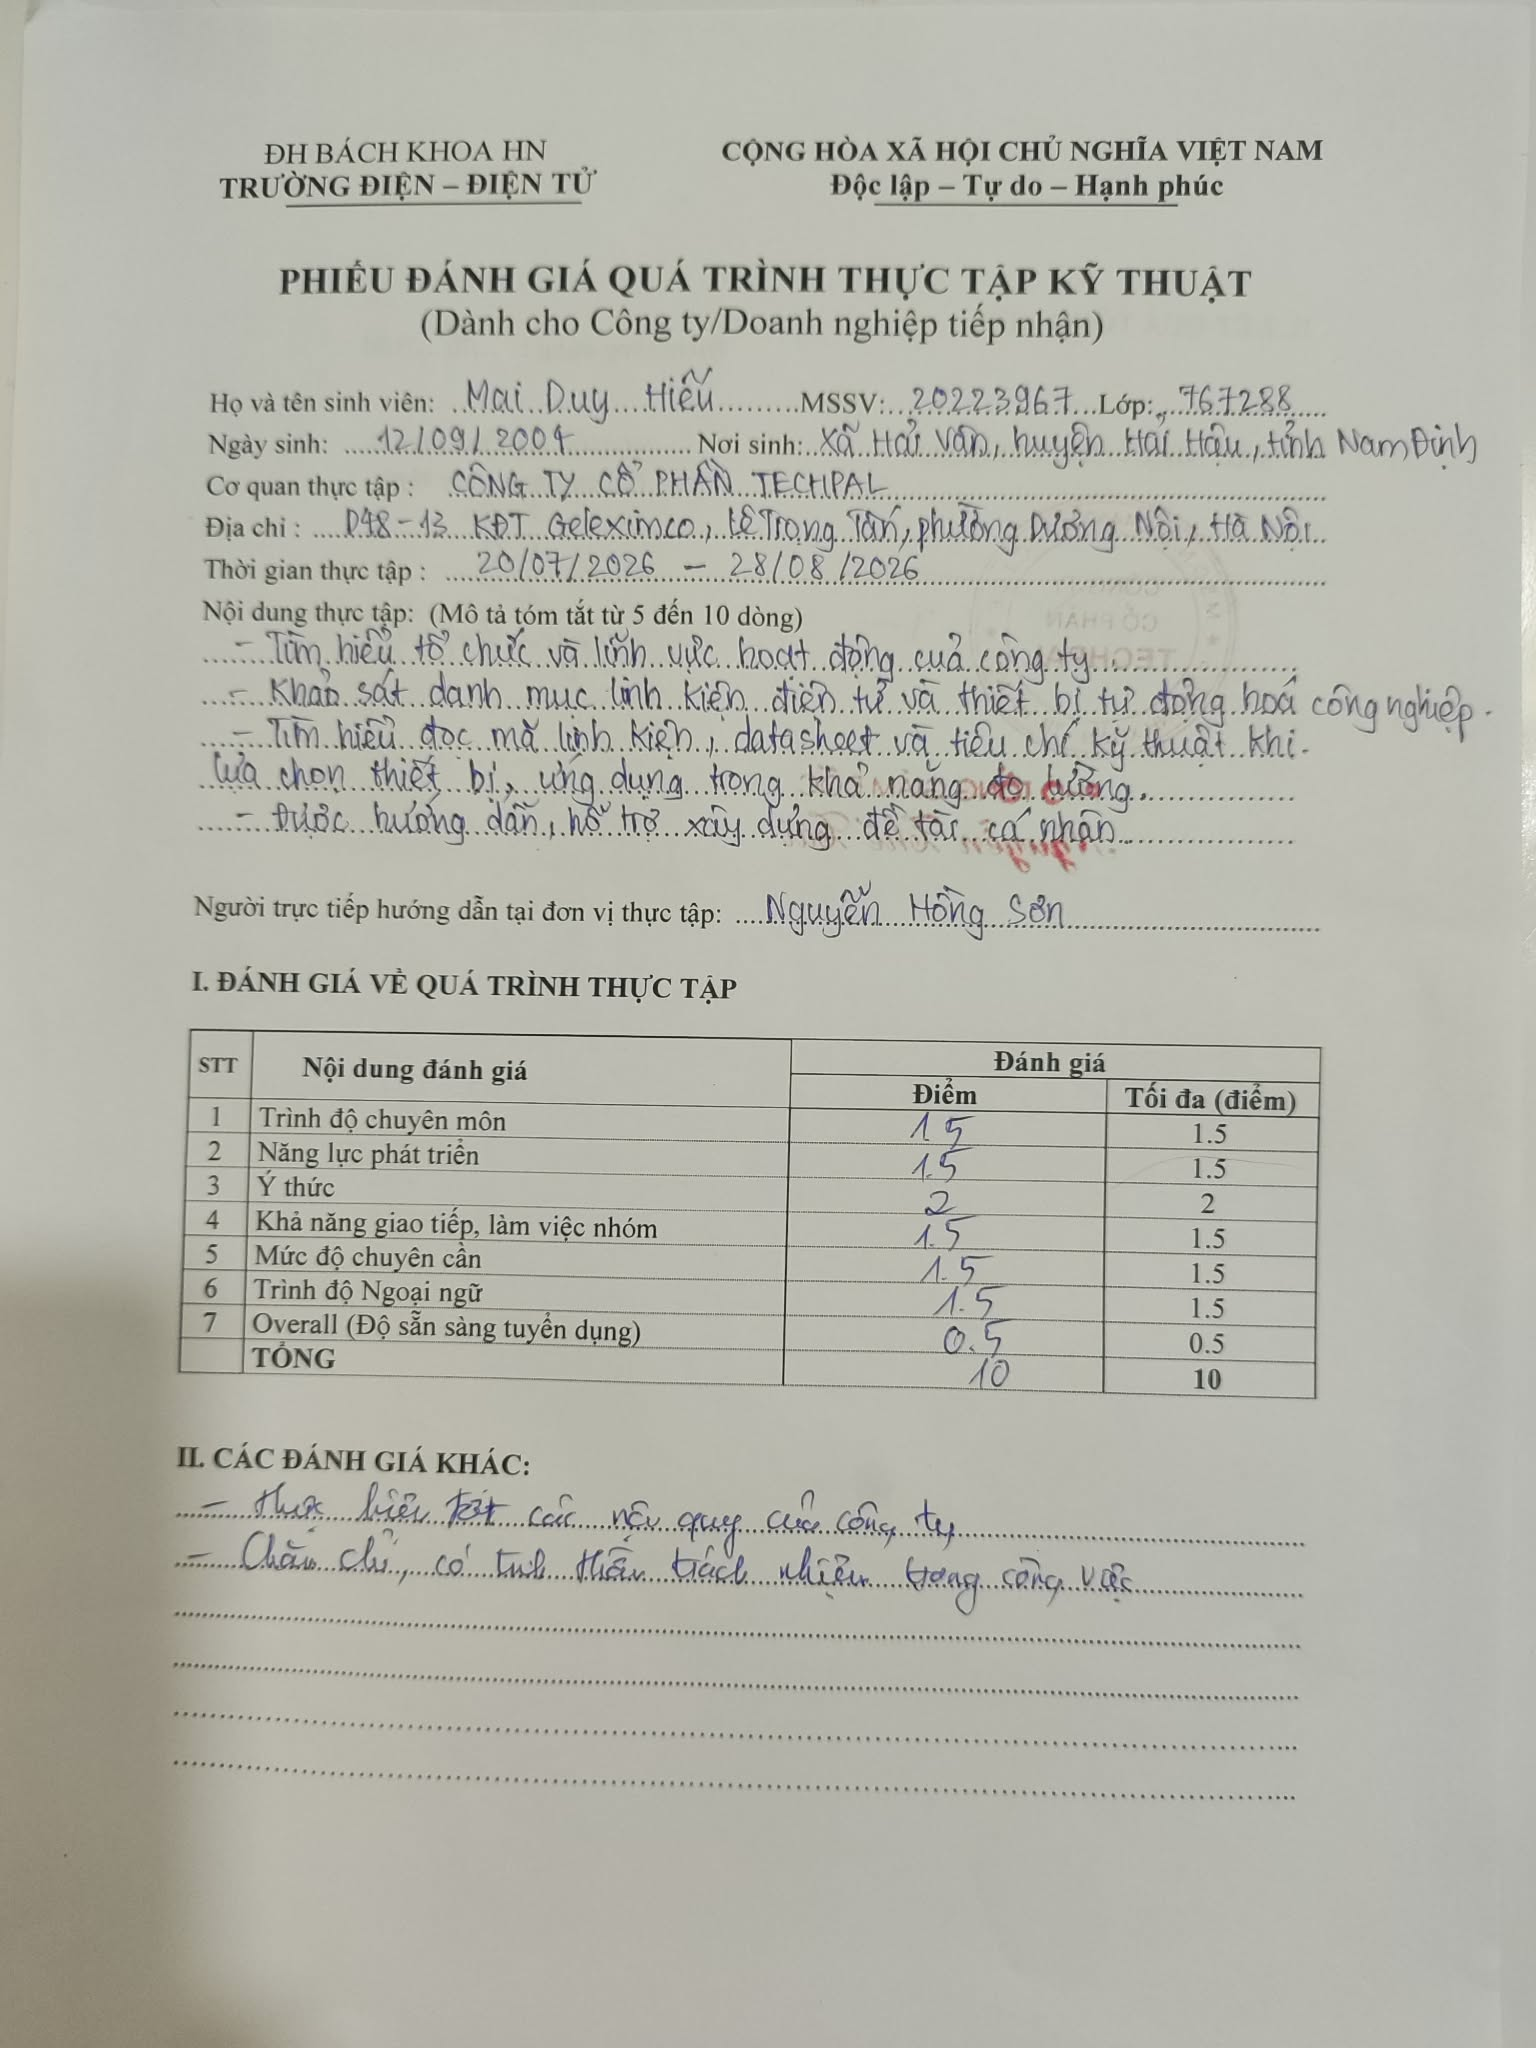
\includegraphics[width=0.82\textwidth]{phieu-danh-gia-trang-1.jpg.png}
\caption{Phiếu đánh giá quá trình thực tập (trang 1)}
\label{fig:phieu-trang-1}
\end{figure}

\begin{figure}[H]
\centering
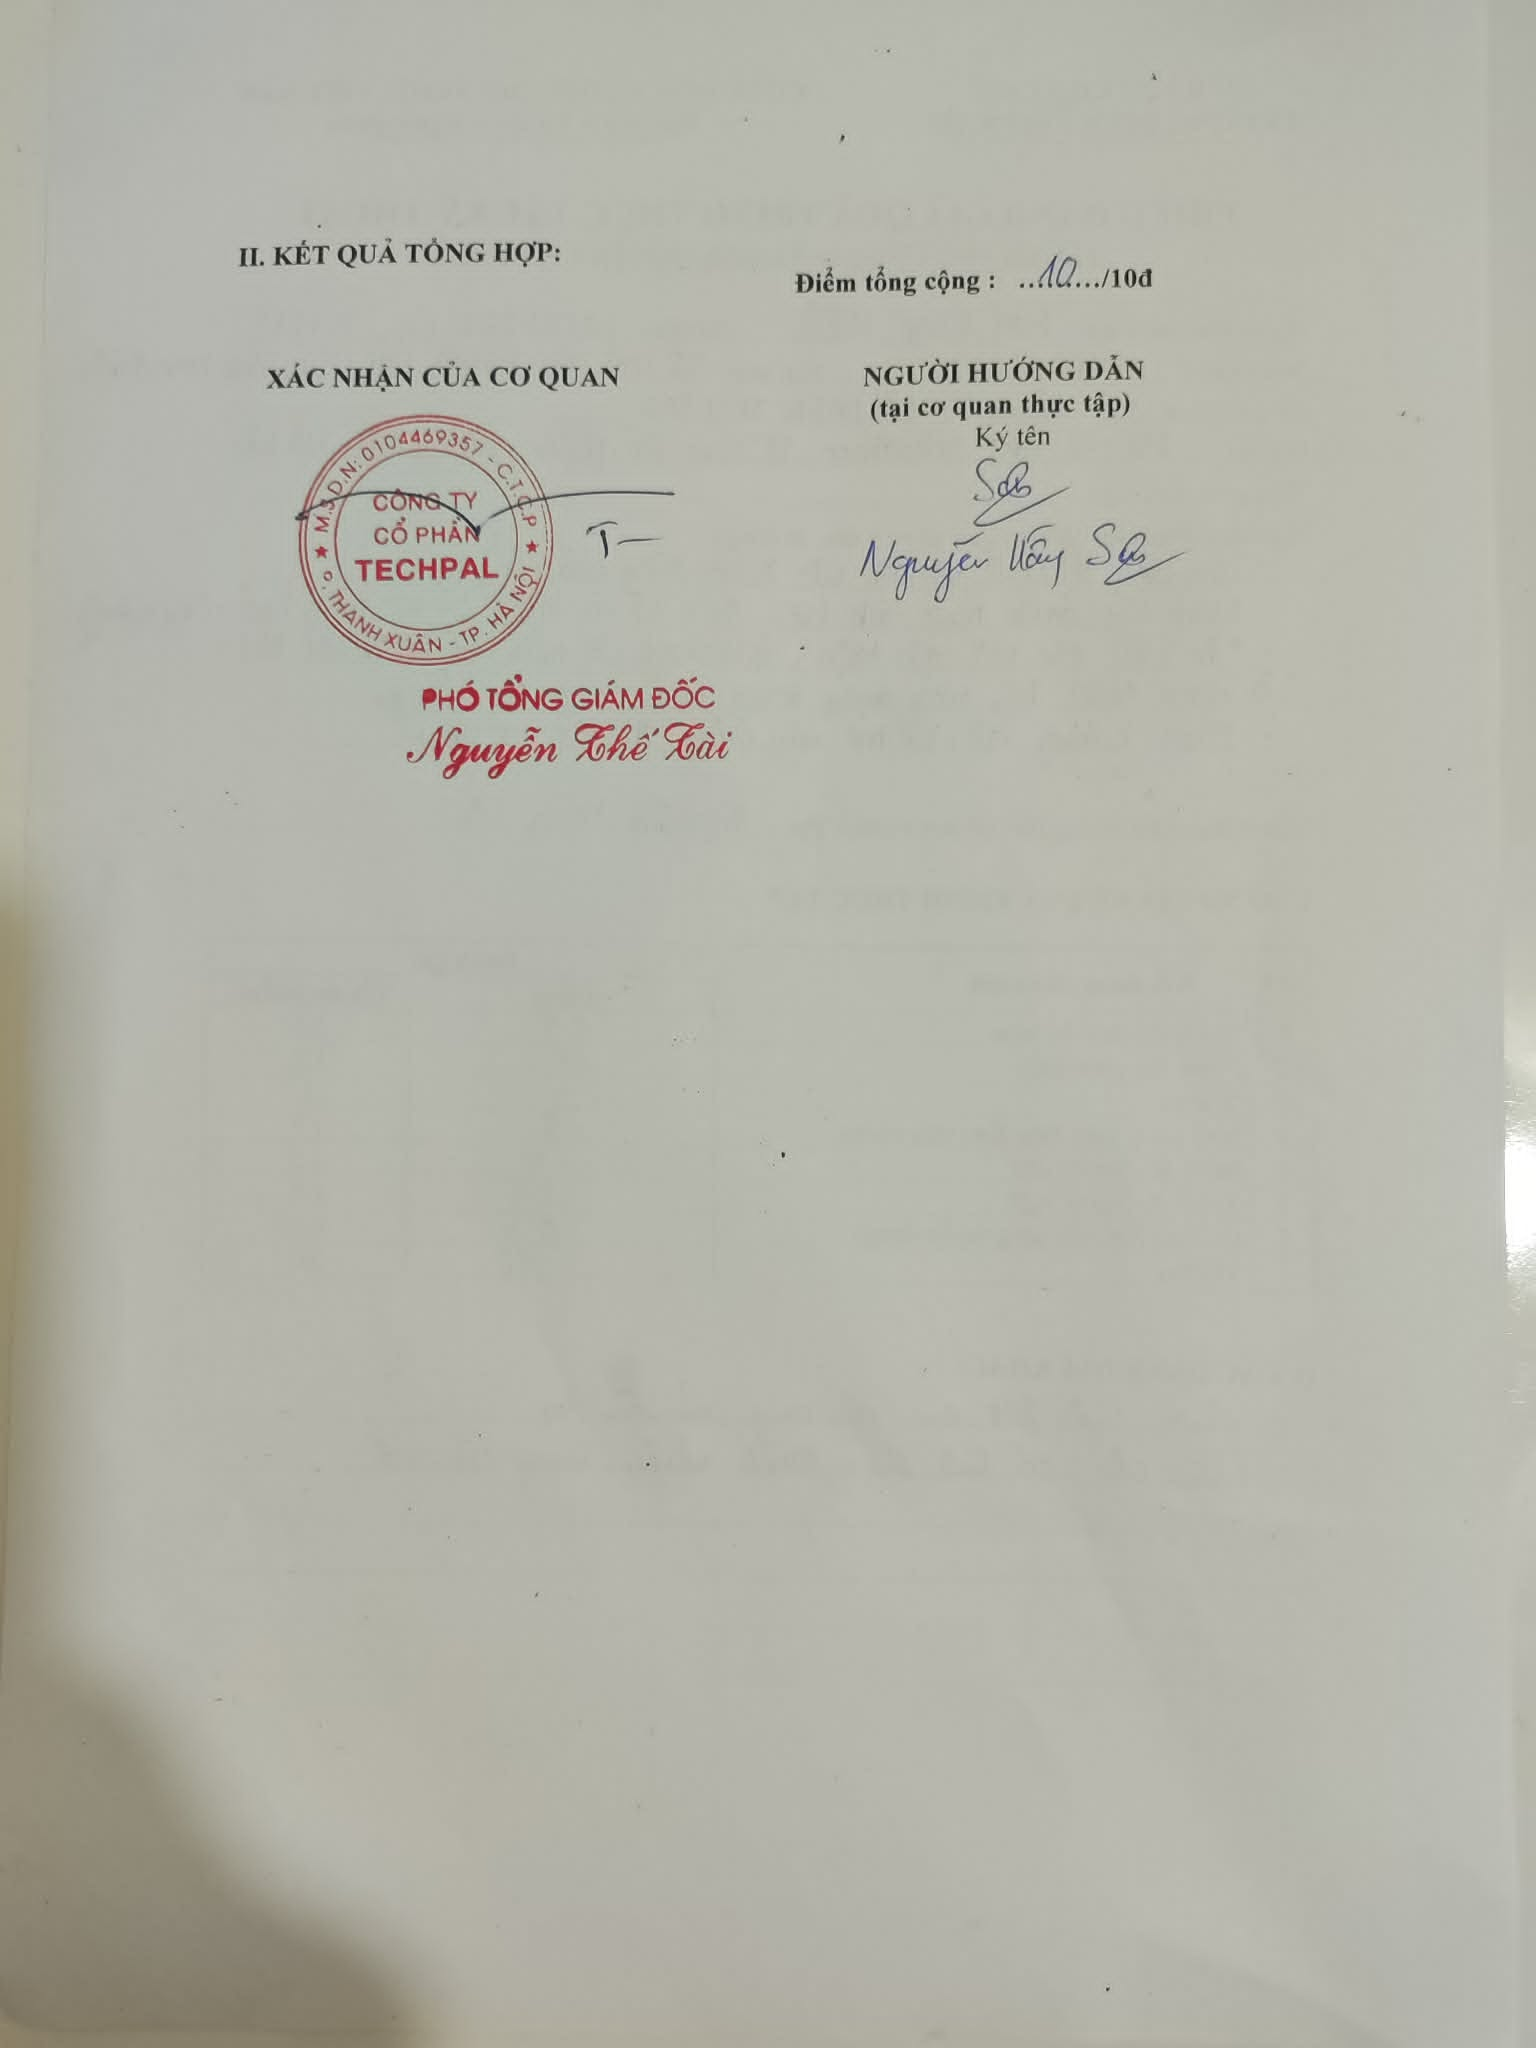
\includegraphics[width=0.82\textwidth]{phieu-danh-gia-trang-2.jpg.png}
\caption{Phiếu đánh giá quá trình thực tập (trang 2)}
\label{fig:phieu-trang-2}
\end{figure}


\end{document}
